\begin{tikzpicture}[font=\bf\sffamily\fontsize{8}{9}\selectfont]
  \def\DCOL{Tomato}
  \def\DCOLx{Tomato}
  \def\DCOL{black!50}
  \def\DCOLx{black!80}
  \def\DCOLS{black}
  \def\ECOLA{black!5}
  \def\ECOLB{black!5}
  \def\ECOLC{Green4!5}
  \def\ECOLD{Green4!5}
  \def\LWD{1pt}
  \def\LWDA{6pt}
  \def\ACOL{black}
  \def\OPC{.8}
  \def\OPCA{.95}
  \def\OPCB{.15}
  \def\CIRC{circle}
  \def\LWT{2pt}
  \def\SCALE{.80}
  \def\LCOL{black!50}
  \node[anchor=south west] (T) at (0,0) {
    \includegraphics[width=3in]{Figures/\EPATH}};

  \node[anchor=south west,label={[text=black,align=center,yshift=-0in,xshift=2.25in]120:{\Large b.} A sample of conditional inference trees\\in inferred \enet (H1N1 HA)}] at ([yshift=0in]T.south east) {
    \begin{tikzpicture}[anchor=center,font=\bf\sffamily\fontsize{8}{8}\selectfont]
      \clip (.93in,-0in) rectangle (-2.85in,-7in);
      \tikzset{xcirc/.style={circle,inner sep=-25pt,dashed,fill=\ECOLB,opacity=\OPC,rounded corners=5pt,draw=\DCOL,line width=\LWD,scale=\SCALE}}
      \def\WDT{2.5in}
      \def\WDTA{2.25in}
      \def\WDTB{2in}
      \def\WDTC{2.40in}
      \coordinate (Z) at (0,0);

      \node[anchor=north west,xcirc,inner sep=-35pt,label={[yshift=.9in,xshift=-.5in,align=center,\LCOL]-90:index\\63}] (P63) at ([xshift=-2.9in,yshift=-.75in]Z) {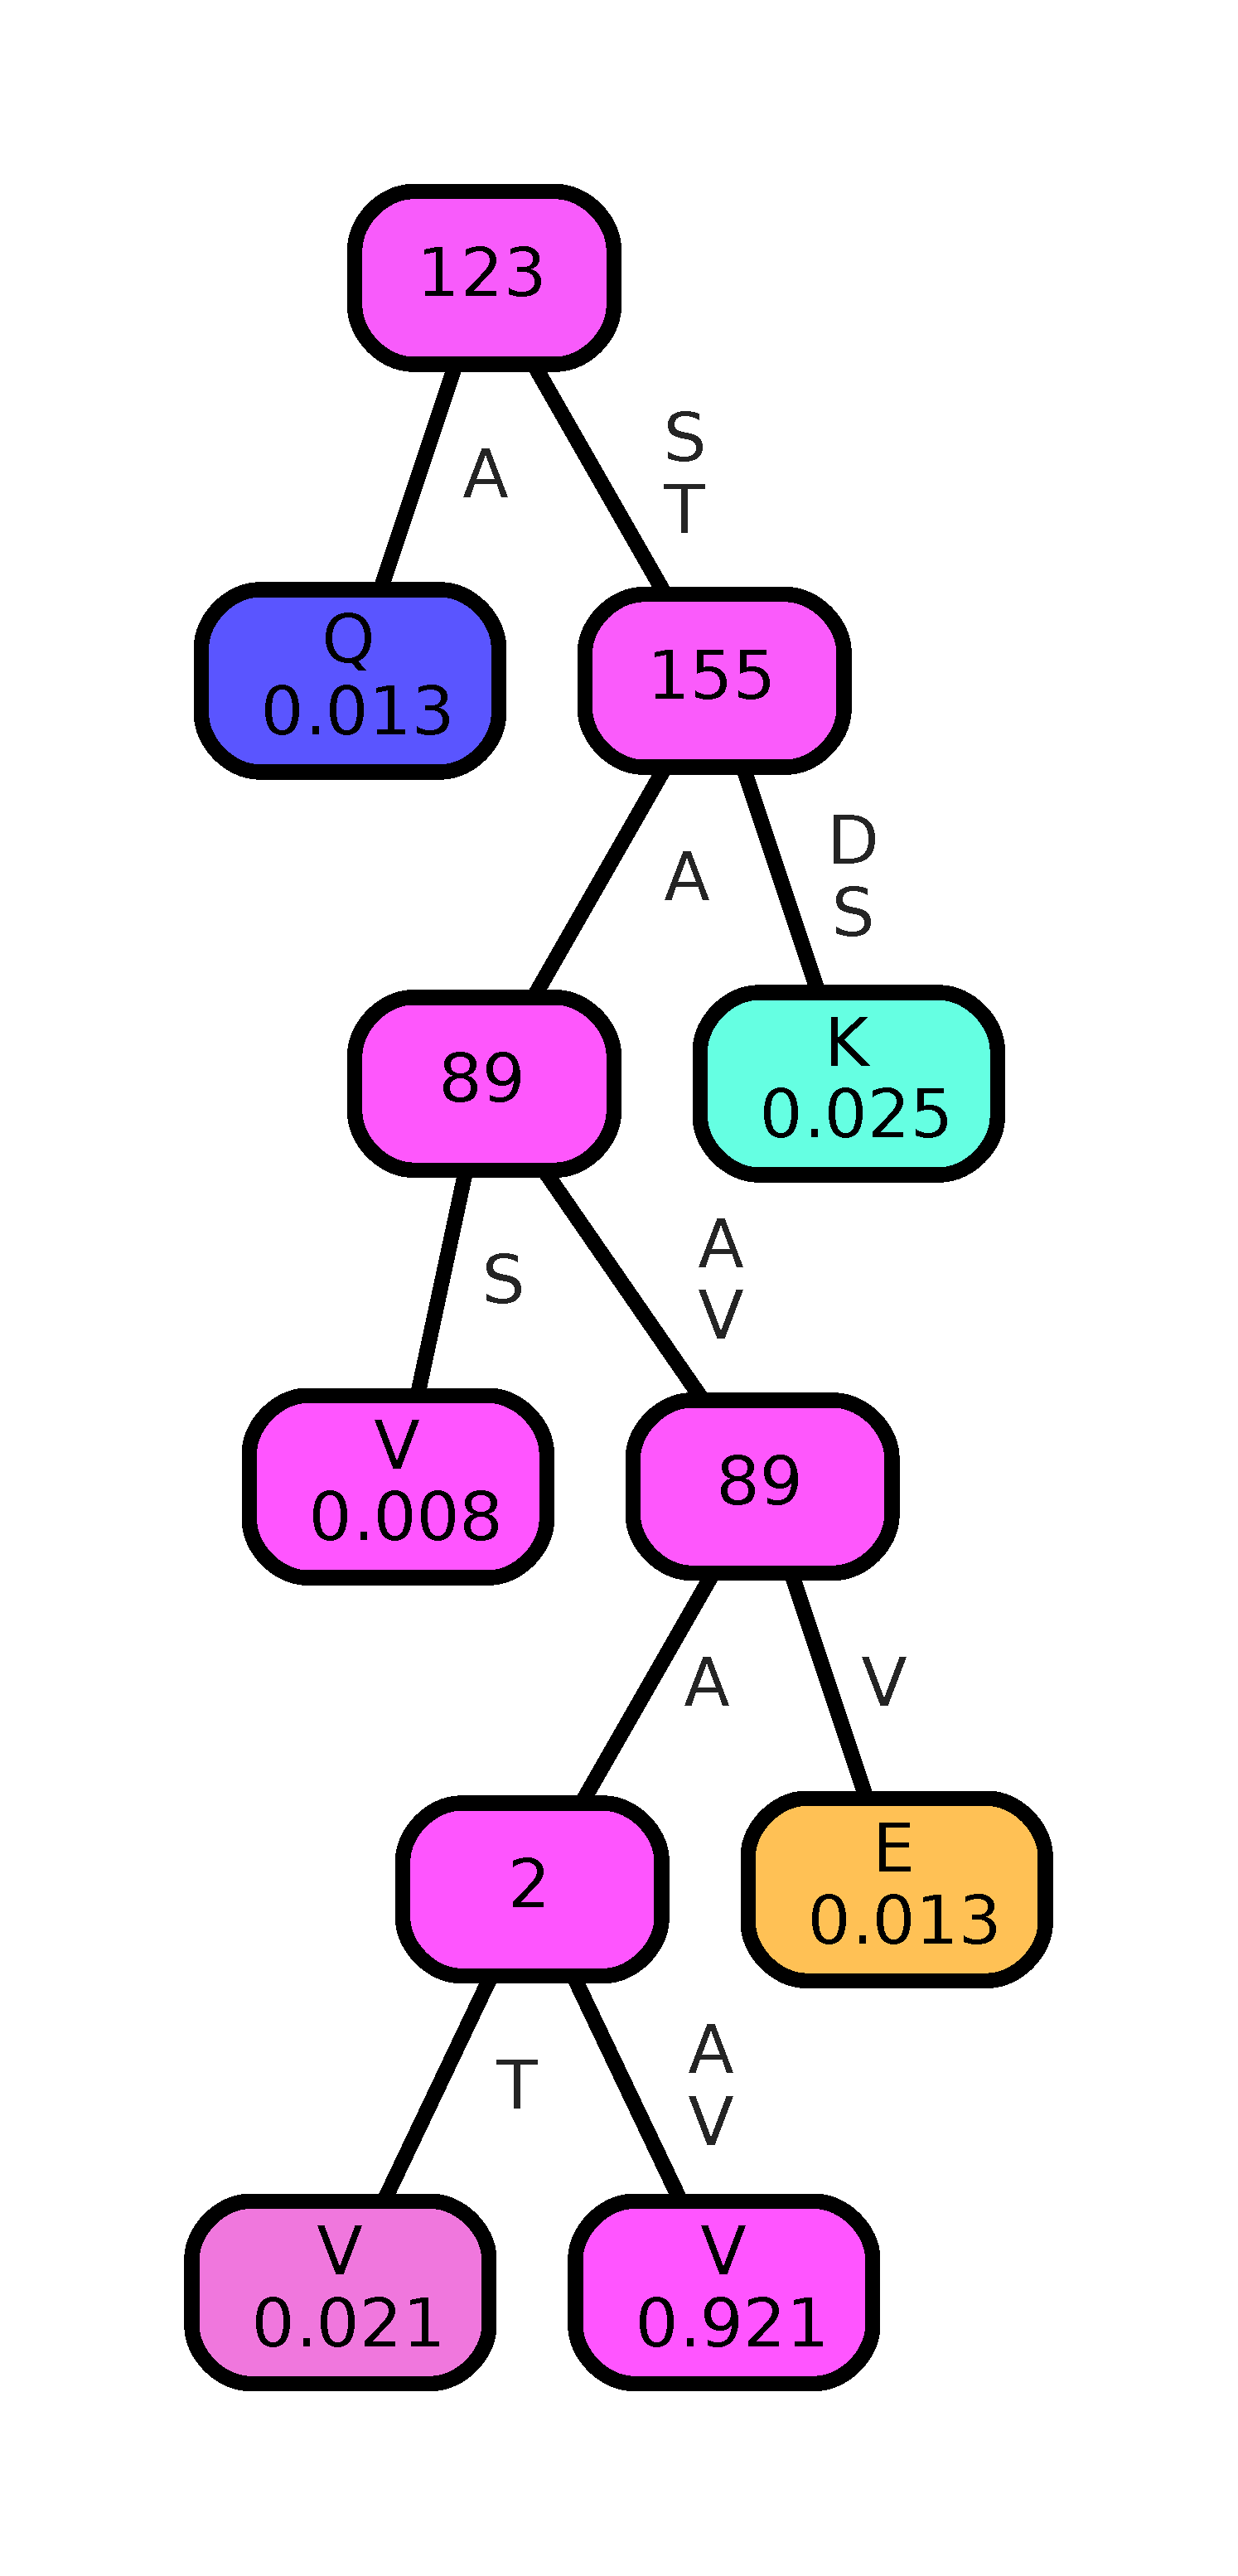
\includegraphics[width=\WDTB]{../qnet_predictions/qnet_models/trees/proc63}}; 

      
      \node[anchor=north,xcirc,inner sep=-20pt,label={[xshift=-.6in,yshift=.7in,align=center,\LCOL]-90:index\\155}] (P155) at (Z) {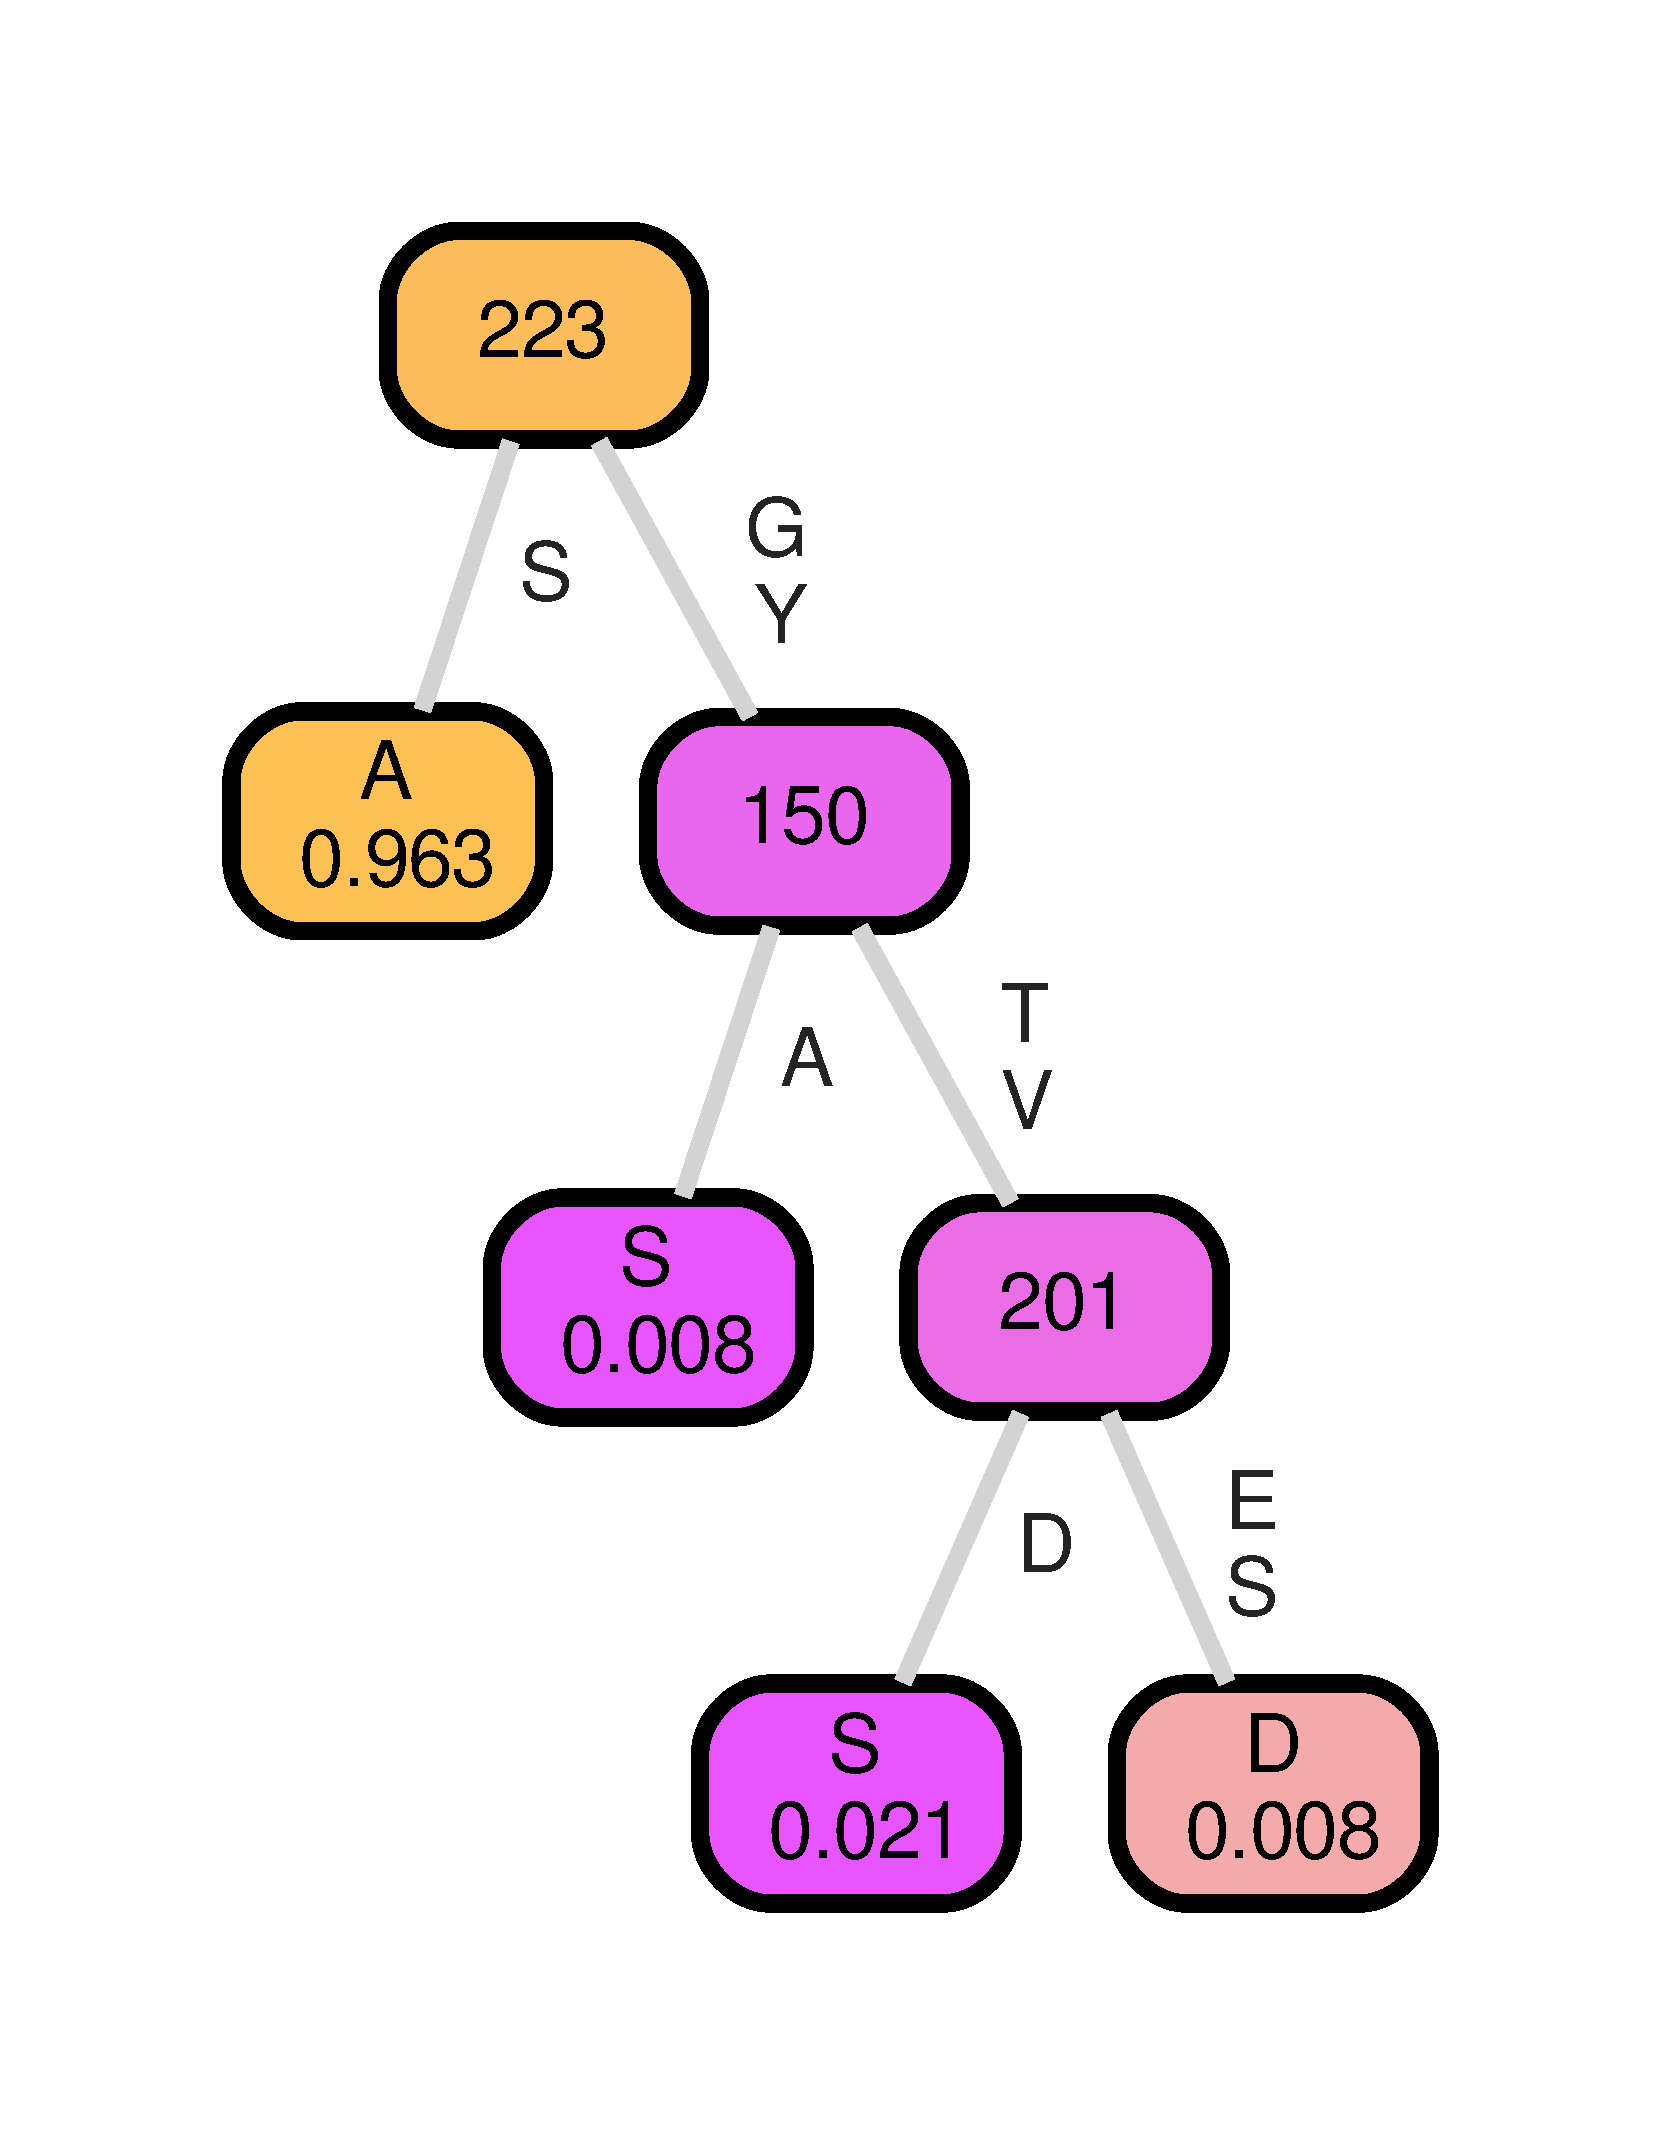
\includegraphics[width=\WDTC]{../qnet_predictions/qnet_models/trees/proc155}};

      \node[anchor=north,xcirc,inner sep=-25pt,label={[yshift=.65in,xshift=-.45in,align=center,\LCOL]-90:index\\14}] (P14) at ([xshift=-2.2in,yshift=-0.8in]P155.south) {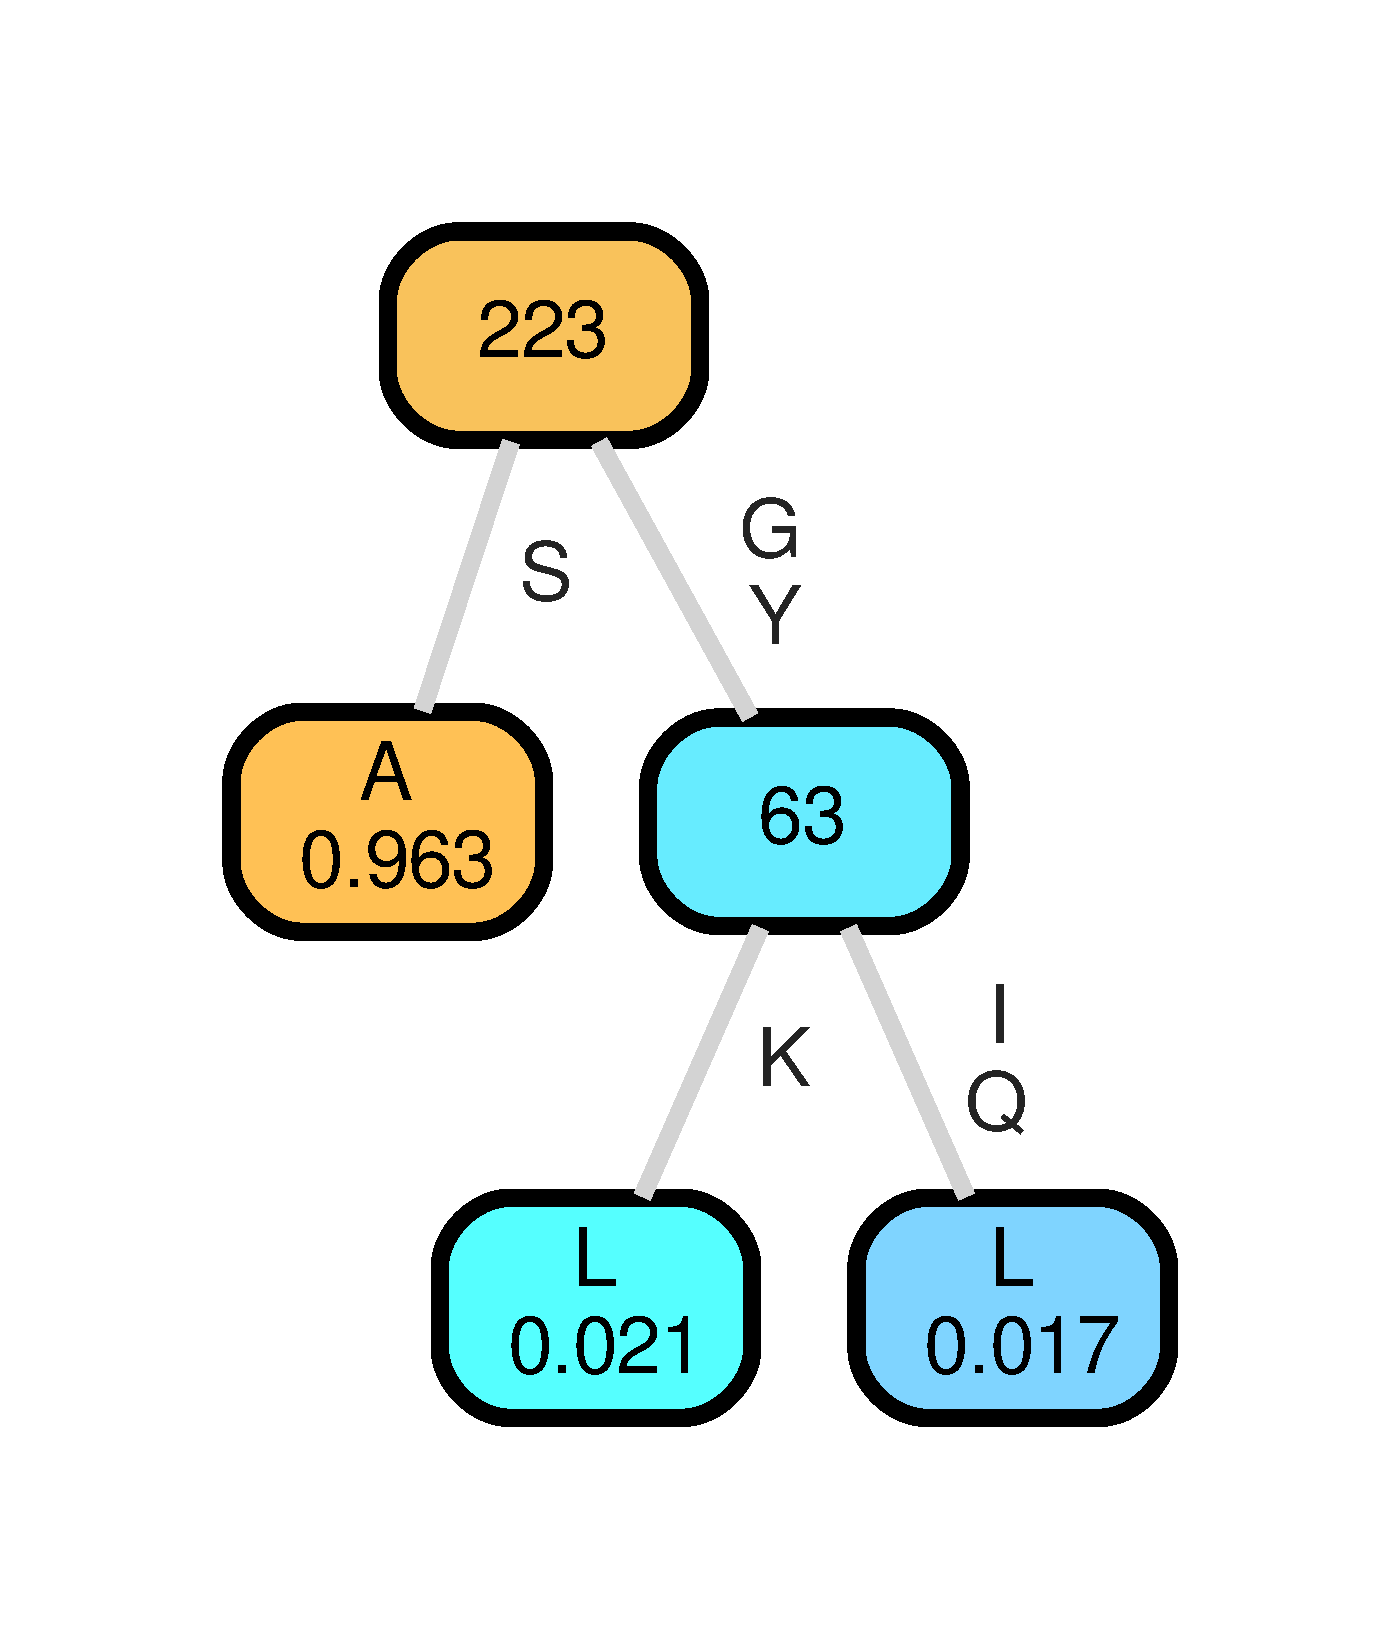
\includegraphics[width=\WDTB]{../qnet_predictions/qnet_models/trees/proc14}}; 
      
      \node[anchor=north,xcirc,inner sep=-25pt,label={[yshift=.6in,xshift=-.5in,align=center,\LCOL]-90:index\\223}] (P223) at ([xshift=-0in,yshift=-0.10in]P155.south) {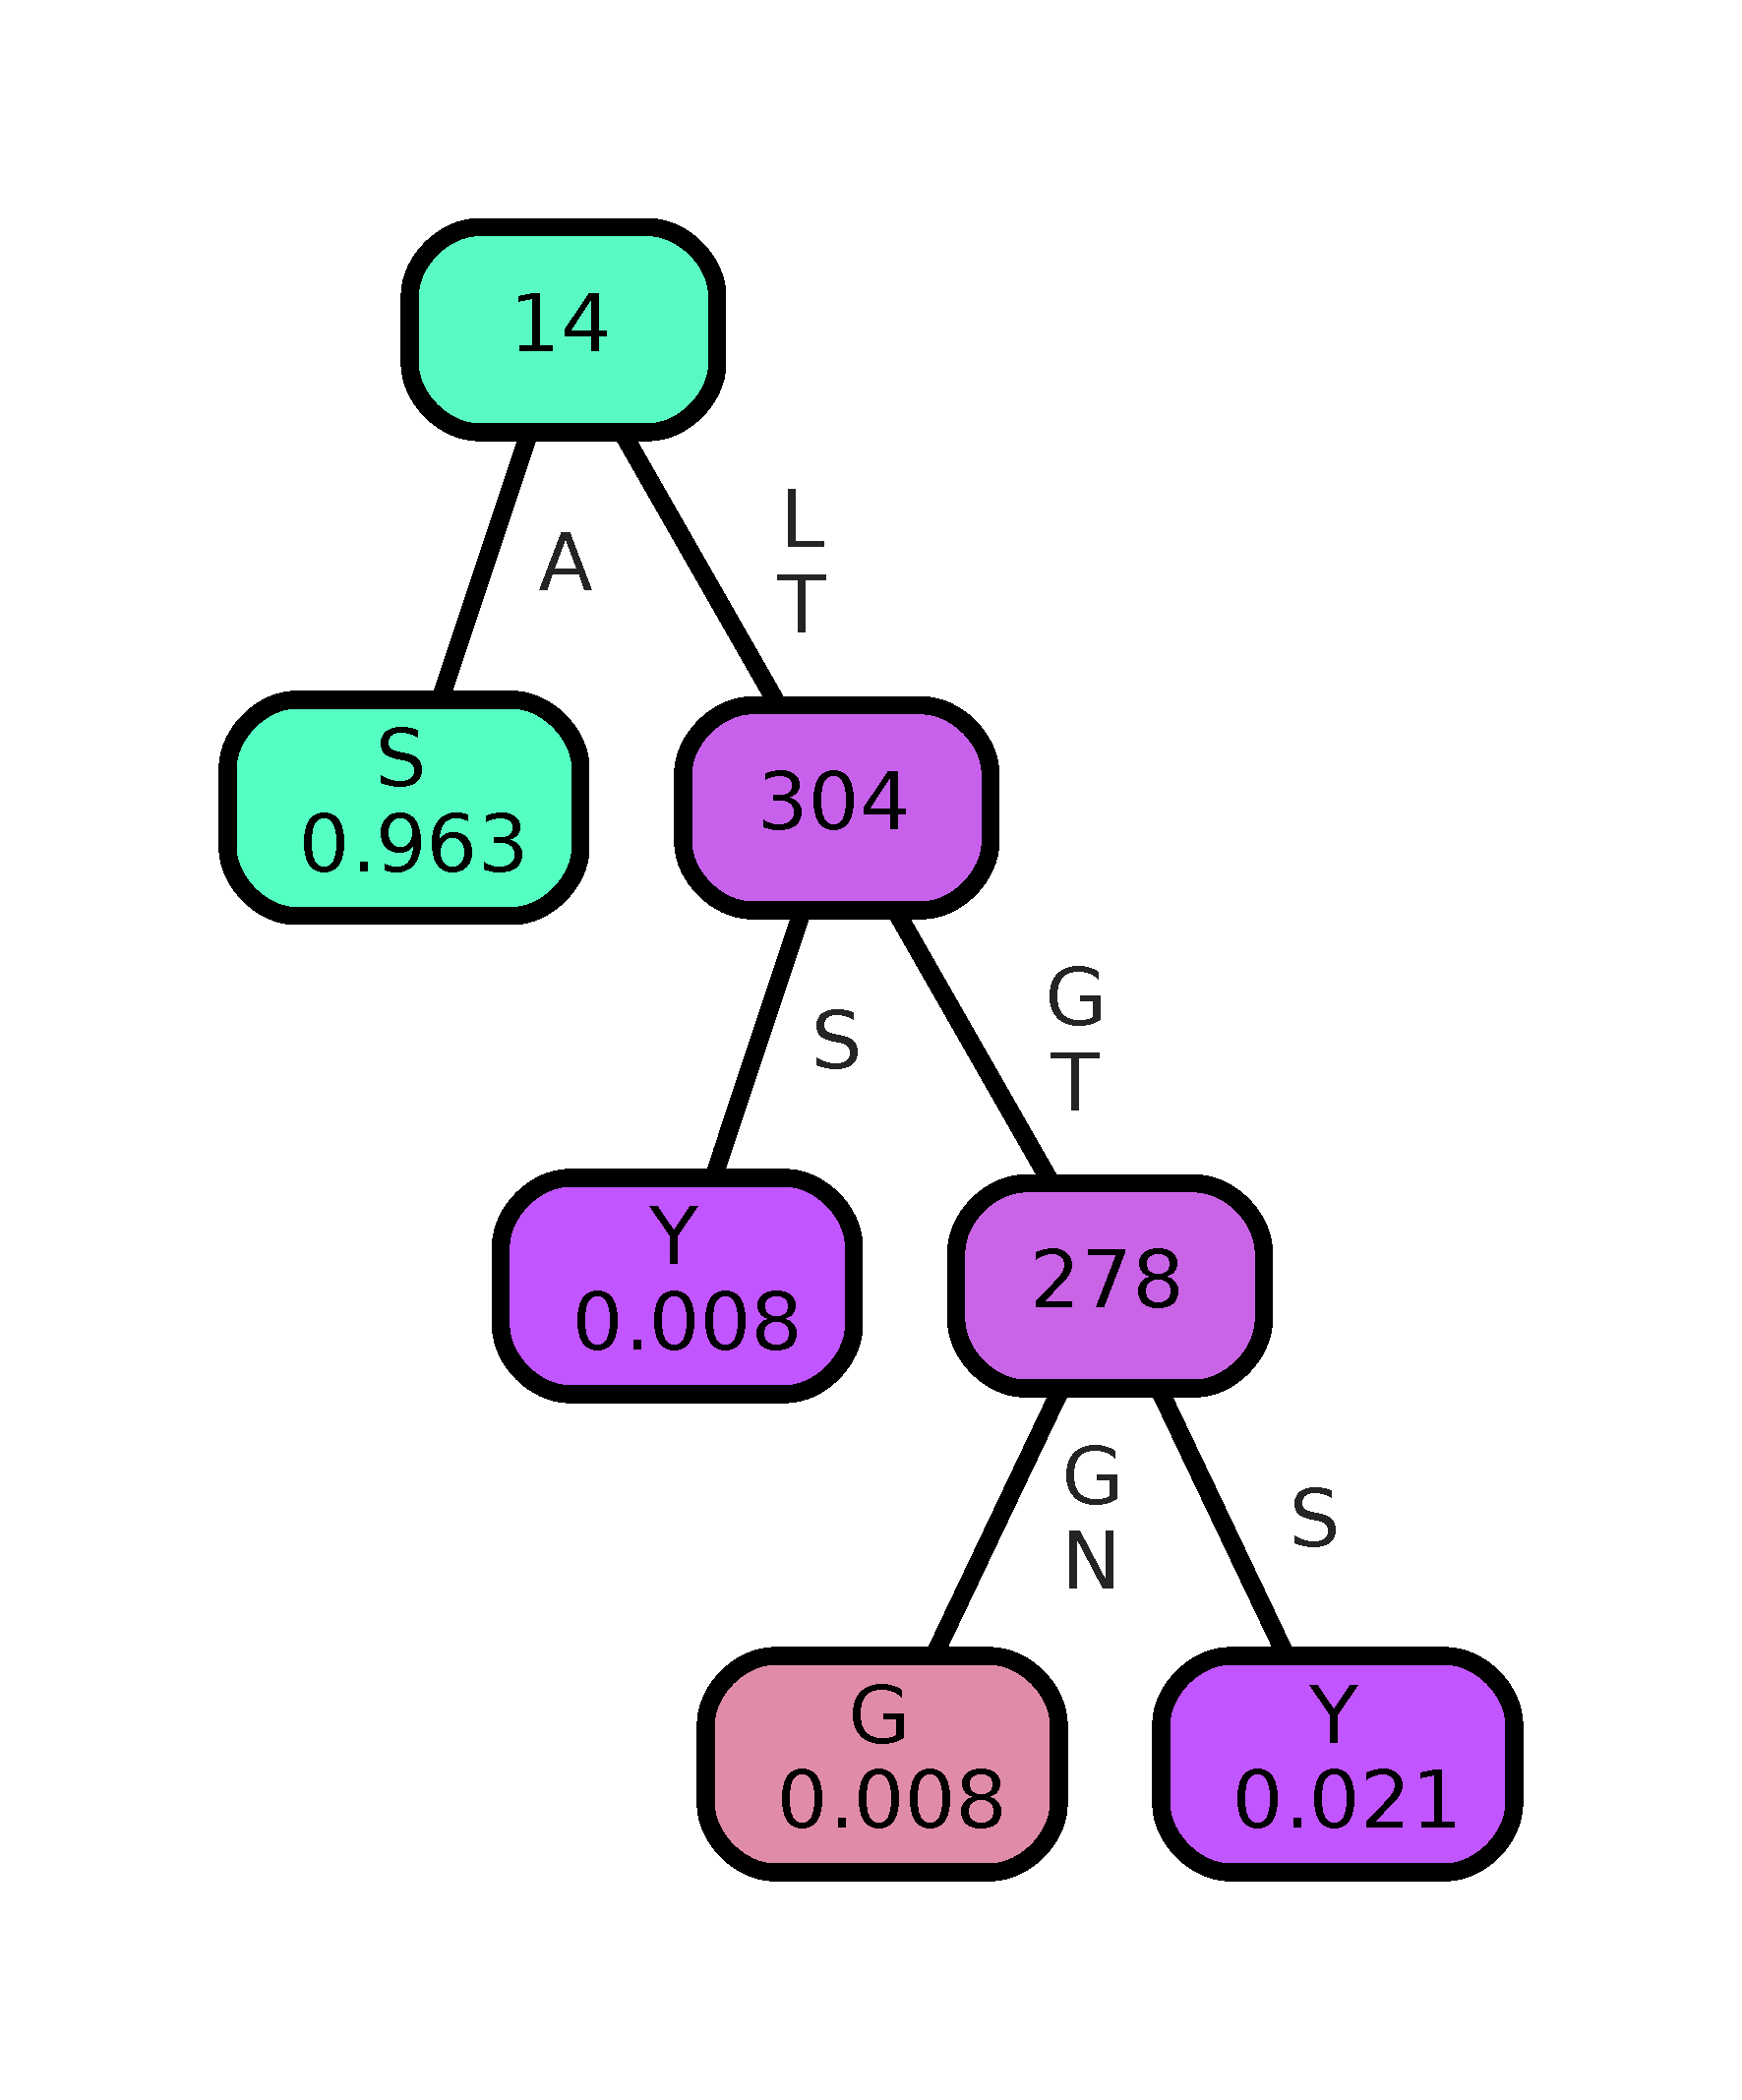
\includegraphics[width=\WDT]{../qnet_predictions/qnet_models/trees/proc223}};


      \node[text width=.13in,  rounded corners=8pt, line width=2pt,,inner sep=10pt,opacity=1,draw=\DCOLx] (X1) at ([yshift=.835in,xshift=.12in]P63) {};
      \draw [line width=\LWT,\DCOLx,-latex,] (X1)  to [out=75,in=140,looseness=1.55]  (P155);

      \node[text width=.13in,  rounded corners=8pt, line width=2pt,inner sep=10pt,opacity=1,draw=\DCOLx] (X2) at ([yshift=.845in,xshift=-.335in]P155) {};
      \draw [line width=\LWT,\DCOLx,-latex,] (X2)  to [out=0,in=60,looseness=1]  (P223);

      \node[text width=.13in,  rounded corners=8pt, line width=2pt,,inner sep=10pt,opacity=1,draw=\DCOLx] (X3) at ([yshift=.0in,xshift=.12in]P14) {};
      \draw [line width=\LWT,\DCOLx,-latex,] (X3)  to [out=150,in=-120,looseness=1.1]  (P63);

      \node[text width=.15in,  rounded corners=8pt, line width=2pt,inner sep=10pt,opacity=1,draw=\DCOLx] (X4) at ([yshift=.88in,xshift=-.34in]P223) {};
      \draw [line width=\LWT,\DCOLx,-latex,] (X4)  to [out=210,in=35,looseness=1.2]  (P14);

      \node[anchor=north,align=left,font=\bf\tt\footnotesize] (N3) at ([yshift=-6.1in,xshift=-1.85in]Z.south) {\bf\sffamily\fontsize{7}{8}\selectfont H1N1 2020-2021\\\bf\sffamily\fontsize{7}{8}\selectfont Haemagglutinin Sequences\\$\cdots$GTSRY{\color{Red1}S}KKFKPEIATRPKVRDQEGR$\cdots$\\$\cdots$GTSKY{\color{Red1}G}KKFMPEIARRPKVRNQEGR$\cdots$\\
        $\cdots$GSSKY{\color{Red1}Y}KRFTPEIVARPKVREQAGR$\cdots$\\
 $\cdots$GSSKY{\color{Red1}Y}KRFTPEIVARPKVREQAGR$\cdots$};

%A/Niger/8327/2020 
%
%A/Parana/10835/2021
%A/Gansu-Xifeng/1143/2021
%A/Sichuan/01208/2021

   \node[anchor=west,align=left,font=\bf\sffamily\fontsize{8}{10}\selectfont] (N4) at ([xshift=0.1in,yshift=.05in]N3.east) {A/Niger/8327/2020 \\
    A/Parana/10835/2021\\
      A/Gansu-Xifeng/1143/2021\\  
      A/Sichuan/01208/2021};

       \draw [ultra thick] ([yshift=.25in,xshift=.01in]N4.west) --++ (-.13in,-.190in);
       \draw [ultra thick] ([yshift=.1in,xshift=.01in]N4.west) --++ (-.13in,-.2in);
       \draw [ultra thick] ([yshift=-0.05in,xshift=.01in]N4.west) --++ (-.13in,-.2in);
       \draw [ultra thick] ([yshift=-.2in,xshift=.01in]N4.west) --++ (-.13in,-.2in);

       \node [align=center,text=IndianRed2,anchor=north] at ([xshift=-2.25in,yshift=-.1in]N4.south) {index 223};

      \node[anchor=west,rounded corners=3pt,align=center] (I1) at ([yshift=-.6in,xshift=.3in]P14.south west) {Color key (mixed colors represent distributions)};


      \definecolor{Acol}{RGB}{255,193,85}
      \definecolor{Dcol}{RGB}{255,255,85}
      \definecolor{Ecol}{RGB}{255,255,85}
      \definecolor{Gcol}{RGB}{136,255,85}
      \definecolor{Icol}{RGB}{85,255,150}
      \definecolor{Kcol}{RGB}{85,255,255}
      \definecolor{Lcol}{RGB}{85,255,255}
      \definecolor{Qcol}{RGB}{111,85,255}
      \definecolor{Scol}{RGB}{231,85,255}
      \definecolor{Tcol}{RGB}{255,85,255}
      \definecolor{Vcol}{RGB}{255,85,255}
      \definecolor{Ycol}{RGB}{255,85,97}
      
      \node[font=\bf\sffamily,anchor=north,rounded corners=3pt,text width=.1in,text height=.1in,fill=Acol,align=center,opacity=\OPC] (I1) at ([yshift=-.05in]I1.south west) {A};
      \node[font=\bf\sffamily,anchor=west,rounded corners=3pt,text width=.1in,text height=.1in,fill=Dcol,align=center,opacity=\OPC] (I1) at ([xshift=.05in]I1.east) {D};
      \node[font=\bf\sffamily,anchor=west,rounded corners=3pt,text width=.1in,text height=.1in,fill=Ecol,align=center,opacity=\OPC] (I1) at ([xshift=.05in]I1.east) {E};
      \node[font=\bf\sffamily,anchor=west,rounded corners=3pt,text width=.1in,text height=.1in,fill=Gcol,align=center,opacity=\OPC] (I1) at ([xshift=.05in]I1.east) {G};
      \node[font=\bf\sffamily,anchor=west,rounded corners=3pt,text width=.1in,text height=.1in,fill=Icol,align=center,opacity=\OPC] (I1) at ([xshift=.05in]I1.east) {I};
      \node[font=\bf\sffamily,anchor=west,rounded corners=3pt,text width=.1in,text height=.1in,fill=Kcol,align=center,opacity=\OPC] (I1) at ([xshift=.05in]I1.east) {K};
      \node[font=\bf\sffamily,anchor=west,rounded corners=3pt,text width=.1in,text height=.1in,fill=Lcol,align=center,opacity=\OPC] (I1) at ([xshift=.05in]I1.east) {L};
      \node[font=\bf\sffamily,anchor=west,rounded corners=3pt,text width=.1in,text height=.1in,fill=Qcol,align=center,opacity=\OPC] (I1) at ([xshift=.05in]I1.east) {Q};
      \node[font=\bf\sffamily,anchor=west,rounded corners=3pt,text width=.1in,text height=.1in,fill=Scol,align=center,opacity=\OPC] (I1) at ([xshift=.05in]I1.east) {S};
      \node[font=\bf\sffamily,anchor=west,rounded corners=3pt,text width=.1in,text height=.1in,fill=Tcol,align=center,opacity=\OPC] (I1) at ([xshift=.05in]I1.east) {T};
      \node[font=\bf\sffamily,anchor=west,rounded corners=3pt,text width=.1in,text height=.1in,fill=Vcol,align=center,opacity=\OPC] (I1) at ([xshift=.05in]I1.east) {V};
      \node[font=\bf\sffamily,anchor=west,rounded corners=3pt,text width=.1in,text height=.1in,fill=Ycol,align=center,opacity=\OPC] (I1) at ([xshift=.05in]I1.east) {Y};

      % \node[font=\bf\sffamily,anchor=north,rounded corners=3pt,text width=.1in,text height=.1in,fill=DarkOrange3!70,align=center,opacity=\OPC] (I1) at ([yshift=-.05in]I1.south) {A};

      % \node[font=\bf\sffamily,anchor=north,rounded corners=3pt,text width=.1in,text height=.1in,fill=SeaGreen2,align=center,opacity=\OPC] (I1) at ([yshift=-.05in]I1.south) {C};

      % \node[font=\bf\sffamily,anchor=north,rounded corners=3pt,text width=.1in,text height=.1in,fill=DodgerBlue2!80,align=center,opacity=\OPC] (I1) at ([yshift=-.050in]I1.south) {G};
    \end{tikzpicture}
  };

  \node [anchor=south west] (L1) at ([yshift=-.2650in]T.north west) {\Large a.};
  \node [anchor=south west] (L2) at ([yshift=-3.25in]T.north west) {\Large c.};
  \node [anchor=south west] (L3) at ([yshift=-5.65in]T.north west) {\Large d.};

\end{tikzpicture}
